\documentclass[toc, titlepaged]{../cs-classes/cs-classes}

\title{Introduction to Computer Vision}
\author{Jean Ponce}

\begin{document}
\begin{abstract}
    This document is Antoine Groudiev's class notes while following the class \emph{Introduction to Computer Vision} (Introduction à la vision artificielle) at the Computer Science Department of ENS Ulm. It is freely inspired by the class notes written by Jean Ponce and Gabriel Fiastre.
\end{abstract}

\section{Introduction and general overview}
\subsection{What is Deep Learning?}
\subsubsection{Neural networks}
\subsubsection{Timeline of Deep Learning}
\subsubsection{Recent applications and breakthroughs}
\subsubsection{Usual setup}
\subsubsection{Required skills}
\subsubsection{Building blocks of deep learning}
\subsubsection{Why deep learning now?}

\subsection{Machine Learning pipeline}
\subsubsection{Cats vs. dogs}
\subsubsection{Typical Machine Learning setup}
\subsubsection{Training objective}

\subsection{Multi-Layer Perceptron}
\subsubsection{Definition}
\subsubsection{PyTorch implementation}
\section{Camera Geometry}

\section{Camera Calibration}
% - Grille de calibration fixe dans le système de coordonnées W (pour world)
% - On attache un deuxième référentiel à la caméra, un des axes étant normal au plan image
% - $P_i$ correspond à un point $p_i$ dans le plan image de la caméra
% - Changement de notation

% - Paramètres extrinsèques, intrinsèques
% - Suppression d'hypothèses pour arriver à une caméra plus générale
% - Pas de rotation du référentiel caméra par rapport au référentiel du monde

% - O(3), SO(3) (orthogonales, orthogonales et det 1)
% - SE(3): matrices 4x4 avec orientation et rotation
\section{Image processing using filters and convolutions}
An image can be interpreted either as a continuous function $f(x, y)$ or as a discrete array $F_{u,v}$. While many applications, especially in image processing, use the discrete array, the intuition and operations are directly derived from the continuous function setup.

\subsection{Filters and convolution}
\subsubsection{Basic filters}
An image can be blurred using a filter, by replacing a point by the average of its neighbors. Blurring an image gives a smoother image, making it easier to compute derivatives. 

% TODO: insert images

\subsubsection{Convolutions}
Given two integrable functions $f, g:\R\to\R$, we can define their convolution as:
\begin{align*}
    f*g: \R&\longrightarrow \R\\
    x&\longmapsto\int_{-\infty}^{+\infty}f(x-t)g(t)dt
\end{align*}
Note that $f*g=g*f$ using a change of variable.

This is the definition of the convolution from a continuous perspective. When dealing with images, we want to apply the convolution to a discrete array. The definition becomes:
\begin{equation*}
    R_{i,j} = (F*G)_{i,j} = \sum_{u,v} F_{i-u, j-v}G_{u,v}
\end{equation*}

% Insert examples of blurring

Convolution follow basic properties:
\begin{description}
    \item[Commutativity] $f*g=g*f$
    \item[Associativity] $(f*g)*h = f*(g*h)$
    \item[Linearity] $(af+bg)*h = af*h + bg*h$
    \item[Shift invariance] $f_t * h = (f*h)_t$
\end{description}
where $f_t(x) = f(x-t)$.
Note that is the only operator that is both linear and shift-invariant.

The convolution can be differentiated:
\begin{equation}
    \label{eq:diff-conv}
    \partfrac{}{x}(f*g) = \partfrac{f}{x}*g
\end{equation}

In practice, we are dealing with discrete and finite arrays; this causes border issues. When applying the convolution with a $K\times K$ kernel, the result is undefined for pixels closer than $K$ pixels from the border of the image. There are multiple ways to solve this issue: \emph{padding} the image with zeros, \emph{cropping} the result, or \emph{wraping around} the image.

\subsubsection{Gaussian filters}
\paragraph*{Bluring images}
Gaussian filters are special filters that are used to blur images. Recall that in one dimension, the Gaussian function is defined as:
\begin{equation*}
    g(x) = \frac{1}{\sqrt{2\pi}\sigma}e^{-\frac{x^2}{2\sigma^2}}
\end{equation*}
In computer vision, we will mostly use the 2-D Gaussian function:
\begin{equation*}
    G(x, y) = \frac{1}{2\pi\sigma^2}e^{-\frac{x^2+y^2}{2\sigma^2}}
\end{equation*}
Note that in the following, we will denote by $1/C$ the normalization constants.

In the continuous setup, blurring a function is achieved by convoluting it with a Gaussian function. In the discrete setup, we can build a matrix kernel that approximates the Gaussian function. Note that the Gaussian function has infinite support, but in actual applications, we can truncate the kernel to a finite size.

Gaussian smoothing oftern provides better results than simple averaging. It is also quite effective to remove the noise in an image. 

\paragraph*{Properties of Gaussian filters}
Gaussian filters remove \say{high-frequency} components from the image; therefore, they are low-pass filters. The quantity of noise removed is proportional to the standard deviation $\sigma$ of the Gaussian kernel. High values of $\sigma$ will remove more noise but will also blur the image more.

\begin{figure}[H]
    \centering
    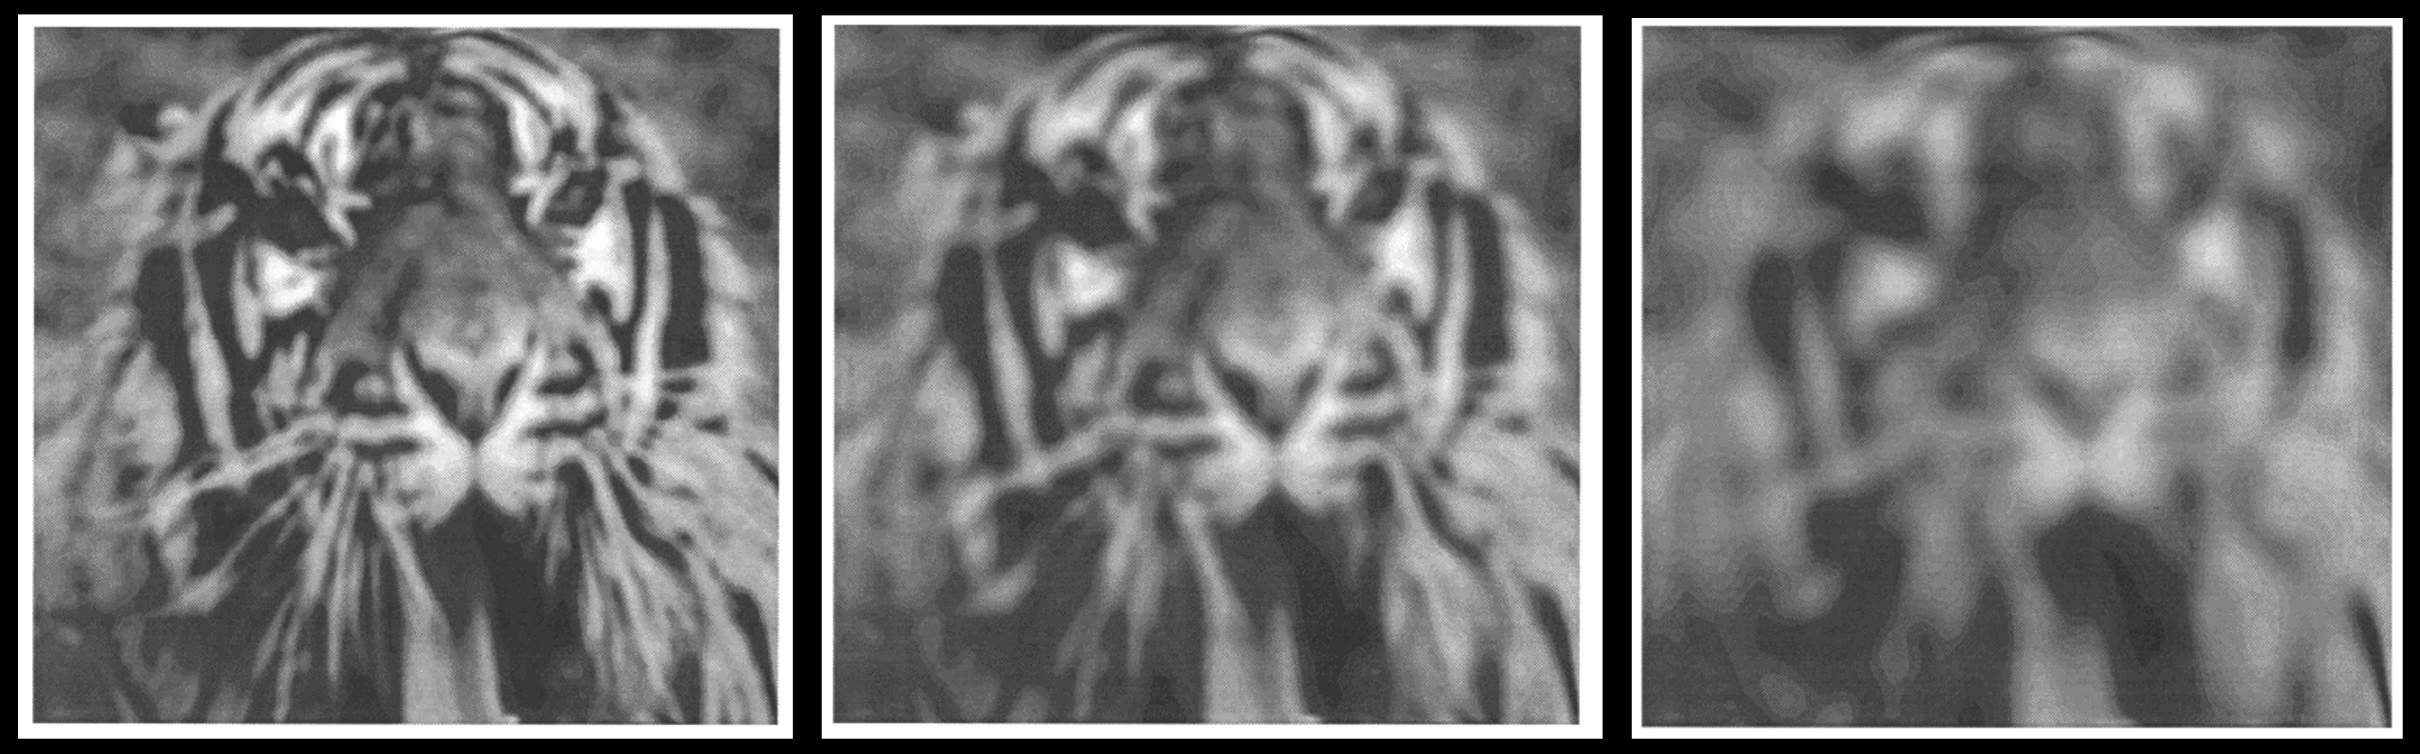
\includegraphics[width=0.8\textwidth]{image-processing/effect-sigma.png}
    \caption{Effect of the standard deviation $\sigma$ on the image.\\ The parameter $\sigma$ is increased from left to right.}
\end{figure}

The combination of 2 Gaussian filters is a Gaussian filter:
\begin{equation*}
    G_{\sigma_1} * G_{\sigma_2} = G_{\sqrt{\sigma_1^2+\sigma_2^2}}
\end{equation*}

Each filter is separable, meaning that we can apply the filter in the $x$ direction and then in the $y$ direction:
\begin{equation*}
    G_\sigma*f = g_{\sigma\rightarrow}*g_{\sigma\uparrow}*f
\end{equation*}
This as a critical implication: filtering with a $n\times n$ Gaussian kernel can be implemented as two convolutions of size $n$, reducing the complexity from $O(n^2)$ to $O(n)$.

\paragraph*{Oriented Gaussian Filters}
By default, $G_\sigma$ smoothes the image by the same amount in all directions. This has the drawback of blurring edges in all directions, which might make edge detection harder later on in the image processing pipeline. If we have some information about preferred directions, we might want to smooth with some value $\sigma_1$ in the direction defined by the unit vector $\begin{bmatrix}a&b\end{bmatrix}$ and by $\sigma_2$ in the direction defined by $\begin{bmatrix}c&d\end{bmatrix}$. This can be achieved using:
\begin{equation*}
    G(x, y) = \frac{1}{C}\exp\left[-\frac{(ax+by)^2}{2\sigma_1^2}-\frac{(cx+dy)^2}{2\sigma_2^2}\right]
\end{equation*}
We can write this in a more compact form using the standard multivariate Gaussian notation:
\begin{equation*}
    G(x, y) = \frac{1}{C}\exp\left[-\frac{X^\tp\Sigma^-1 X}{2}\right] \quad\text{where}\quad X = \begin{bmatrix}
        x\\ y
    \end{bmatrix}
\end{equation*}
The two (orthogonal) directions of filtering are given by the eigenvectors of $\Sigma$, the amout of smoothing is given by the square root of the corresponding eigenvalues of $\Sigma$.

% Insert illustrations

\subsection{Image derivatives}
We will see in the next chapter a variety of techniques to solve the \emph{edge detection problem}. A building block of such methods are \emph{image derivatives}: intuitively, we want to be able to measure how much the contrast of the image change locally. Peaks in contrast variation can be somehow interpreted as being close to edges, since this would be the point where the contours of the object contrast with the background.
\subsubsection{Finite differences}

Therefore, we want to compute at each pixel $(x, y)$ the derivates. In the discrete case, we could take the difference between the left and right pixels:
\begin{equation*}
    \partfrac{I}{x} \simeq I[i+1, j] - I[i-1,j]
\end{equation*}
This is equivalent as convoluting the image by:
\begin{equation*}
    \partial_x = \begin{bmatrix}
        1&0&-1
    \end{bmatrix}
\end{equation*}
The problem of this method is that it increases noise. Consider a noise model in which the actual image $I$ can be decomposed as the sum of the true, noiseless, image $\hat{I}$, and a noise $n$, following for instance a normal distribution. When then have $I=\hat{I}+n$, and we obtain:
\begin{equation*}
    \underbrace{I[i+1,j]-I[i-1,j]}_{\text{Actual image values}}=\underbrace{\hat{I}[i+1,j]-\hat{I}[i-1,j]}_{\text{True difference}}+\underbrace{n_++n_-}_{\text{Noises}}
\end{equation*}
Where $n_+-n_-$ follows a normal distribution of larger variance, providing therefore more noise on the derivate image.

\subsubsection{Smooth derivatives}
A solution is to first smooth the image by a Gaussian $G_\sigma$, and \emph{then} take derivatives:
\begin{equation*}
    \partfrac{f}{x} \simeq \partfrac{G_\sigma*f}{x}
\end{equation*}
Applying the differentiation property of the convolution \eqref{eq:diff-conv}:
\begin{equation*}
    \partfrac{f}{x} \simeq \partfrac{G_\sigma}{x}*f
\end{equation*}
Therefore, taking the derivative in $x$ of the image can be done by applying a convolution with the derivative of a Gaussian:
\begin{equation*}
    \partfrac{G_\sigma}{x}=\frac{1}{C}\cdot x\exp\left[-\frac{x^2+y^2}{2\sigma^2}\right]
\end{equation*}
Another crucial property is that the Gaussian derivative is also separable, reducing drastically the computational cost.

% TODO: insert graph of 1D/2D derivative of Gaussian

Smoothing before the derivative improves the results by reducing the noise, but still blurs away the edge information. In practice, there is always a tradeoff to find between smoothing and good edge localization.

\subsubsection{Beyond smooth derivatives}
Other methods are sometimes used in practice to overcome the limitations detailled above. \emph{Directional derivatives} are the equivalent of directional smoothing; we output the following quantity
\begin{equation*}
    \cos\theta\partfrac{G_\sigma}{x}+\sin\theta\partfrac{G_\sigma}{y}
\end{equation*}
This allows to avoid the smoothing of the edges while keeping the differentiation in directions that matter.

Second-order methods can also prove effective. This is a non-separable method, approximated by a difference of Gaussians. The output of the convolution is the Laplacian of the image; zero-crossing correspond to edges:
\begin{equation*}
    \nabla^2G_\sigma(x,y) = \partfrac{^2G_\sigma(x,y)}{x^2} + \partfrac{^2G_\sigma(x,y)}{y^2}
\end{equation*}
\section{Edge Detection}
The edge detection problem aims at identifying the \emph{edges} inside an image; this requires a proper definition of \say{edge}, which often depends on the method used to compute it. In general, an edge is a place where the intensity of the image changes abruptly. 

The edge detection problem is a fundamental problem in computer vision, as it is the first step in many image processing tasks. The main motivation behind edge detection is the idea that the edges of an image contain important information about the structure of the objects in the scene. If the brightness of an image changes abruptly, it is likely that other properties of the image also change abruptly at that point, and specifically higher-level properties. Edges define the boundaries of objects in the image; they are caused by change of texture, color, depth, or illumination, which all are important cues for the semantic interpretation of the image.

\subsection{Gradient-based edge detection}
Intuitively, an edge is a discontinuity of intensity in some direction; like explained previously, it could be detected by looking for place where the derivatives of the iamge have large values.

Gradient-based edge detectors run into three major issues:
\begin{description}
    \item[Change of scale] The gradient magnitudes at different scales are different: which one should we choose? This reflects a fundament problem in computer vision, which is the necessity to select a threshold under which edges are \say{too small} to be considered.
    \item[Thick countours] The gradient magnitude is large along thick trails: how do we identify the significant points?
    \item[Continuity] Simple edge detection algorithms will produce non-continuous lines, which does not fit our high-level understanding of edges. How do we link the relevant points up into curves?
\end{description}

Another way to detect an extremal first derivative is to look for a null second derivative. In practice, applying a Laplacian method always require smoothing with a Gaussian kernel first. The method goes as follows: smooth the image, apply the Laplacian, and mark the zero points where there is a sufficiently large derivative -- that is enough contrast.

\subsection{The Canny edge detector}
\subsubsection{Introduction}
The Canny edge detector is a multi-step edge detection algorithm, providing a good trade-off between the three issues mentioned above. Instead of simply thresholding the gradient magnitude -- which would lead to thick contours and discontinuous lines -- the Canny edge detector track edges using a process called \emph{hysteresis}.

The starting point of Canny's results is the observation that gradient magnitude does enhance the edges, but runs into two main issues:
\begin{itemize}
    \item using a single threshold either leads to too many edges, or too few edges;
    \item even if we find a good threshold, the edges remain poorly localized, i.e. too thick.
\end{itemize}
Therefore, Canny's edge detector uses two standard tools to address these issues, \emph{non-maximum suppression} and \emph{hysteresis}.

\subsubsection{Non-local maxima suppression}
The goal of Non-Maximum Suppression (NMS) is to thin the edges; the idea is to keep only the pixels that correspond to a maximum in one of the directions of the gradient. If in all directions, the pixel is not a maximum, then it is likely to be a thick contour, and should be removed. Conversely, if the pixel is a maximum in one direction, it is likely to be at the center of the edge stroke, and should be kept.
\begin{figure}[H]
    \centering
    \begin{minipage}{.4\textwidth}
        \centering
        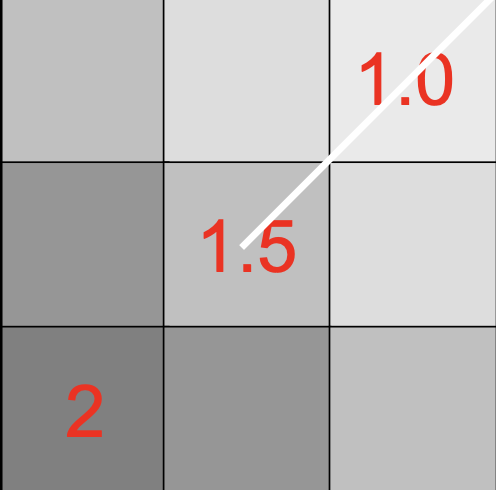
\includegraphics[width=.6\textwidth]{edge-detection/nms-1.png}
        \caption*{Gradient magnitude at center is lower than a neighbor}
    \end{minipage}
    \begin{minipage}{.4\textwidth}
        \centering
        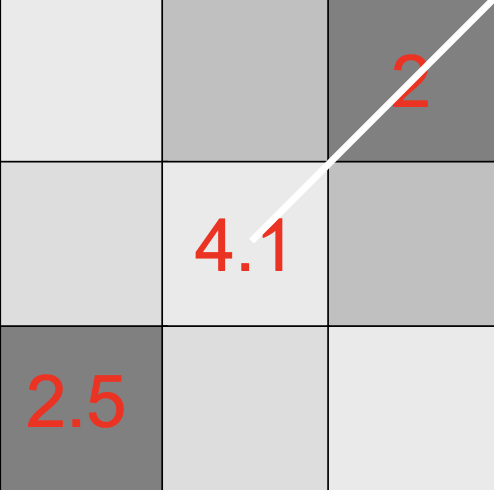
\includegraphics[width=.6\textwidth]{edge-detection/nms-2.png}
        \caption*{Gradient magnitude is a local maximum}
    \end{minipage}
\end{figure}
This creates a mask of the image, where only the local maxima are kept. Applying this mask to the gradient magnitude image will therefore thin the edges.
\begin{figure}[H]
    \centering
    \begin{minipage}{.3\textwidth}
        \centering
        
\includegraphics[width=.8\textwidth]{edge-detection/edge-1.png}
    \end{minipage}
    \begin{minipage}{.3\textwidth}
        \centering
        
\includegraphics[width=.8\textwidth]{edge-detection/edge-2.png}
    \end{minipage}
    \caption{The left image shows the gradient magnitude of an image; on the right, the mask provided by NMS and its application to the gradient.}
\end{figure}

\subsubsection{Hysteresis thresholding}
As stated previously, lower thresholds keep important details, but also keep a lot of noise; higher thresholds remove the noise, but also remove important information about the edges. The idea of hysteresis thresholding is to use two thresholds, a lower and an upper one, to keep only the pixels that are above the upper threshold, or connected to a pixel above the upper threshold. This allows to keep the important details, while removing the noise (i.e. the pixels that are not connected to the edges). Hysteresis also tend to produce continuous edges, since we track the edges by following the pixels that are connected to the edges.
\begin{figure}[H]
    \centering
    \begin{minipage}{.6\textwidth}
        \centering
        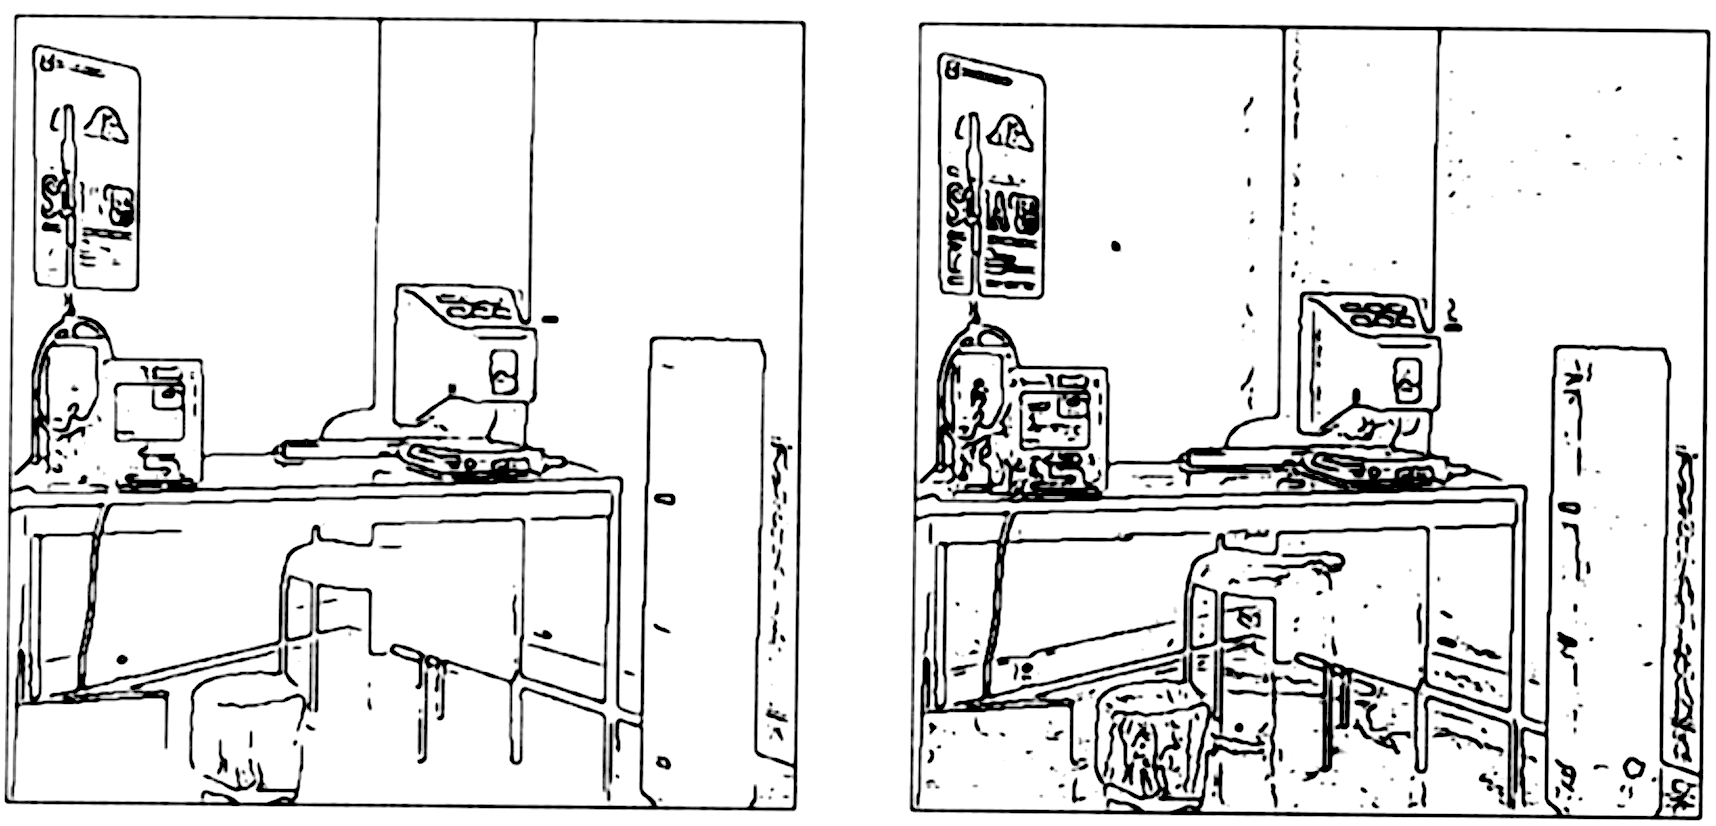
\includegraphics[width=.9\textwidth]{edge-detection/thresholds.png}
        \caption*{Two thresholds: $t=15$ and $t=5$}
    \end{minipage}
    \begin{minipage}{.3\textwidth}
        \centering
        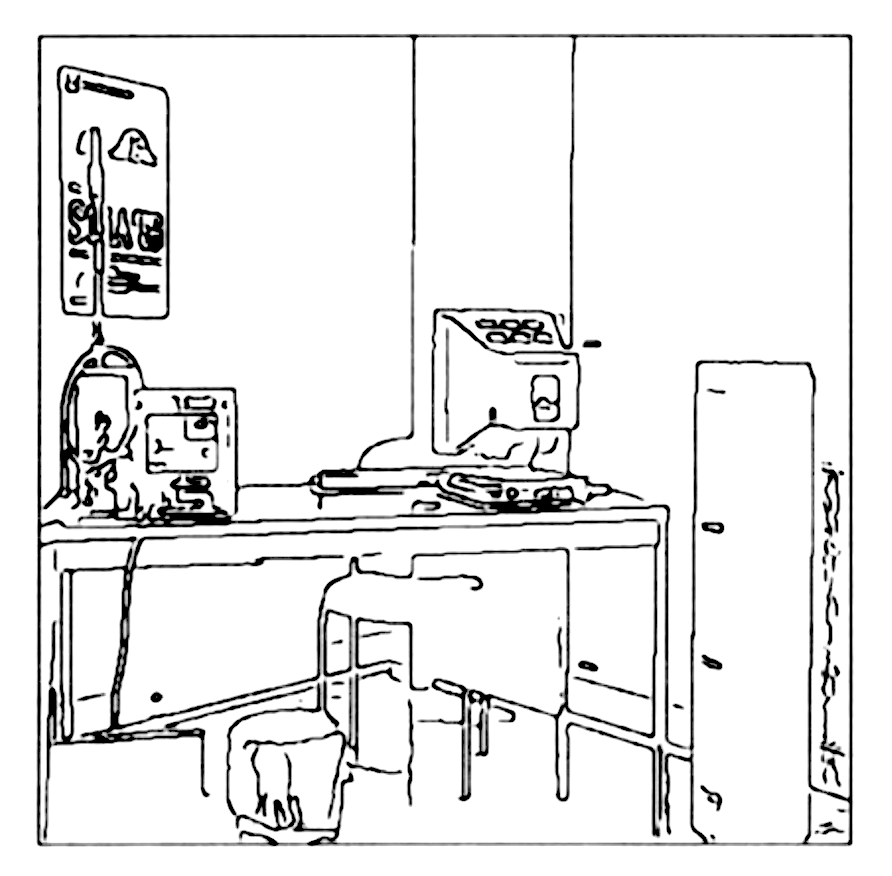
\includegraphics[width=.9\textwidth]{edge-detection/hysteresis.png}
        \caption*{Hysteresis thresholding}
    \end{minipage}
\end{figure}

Hysteresis thresholding can be implemented using a depth-first search algorithm, which will track the pixels connected to the edges. The algorithm goes as follows:
\begin{enumerate}
    \item Keep a set $E$ of the edges for which you have to visit neighbours;
    \item Initialize $E$ with the edges corresponding to the most discriminative threshold;
    \item Until $E$ is empty:
    \begin{itemize}
        \item Extract an edge $e$ from $E$; if $e$ has already been visited, skip it;
        \item For each neighbour $e'$ of $e$:
        \begin{itemize}
            \item If $e'$ is a considered edge using the less discriminative threshold, add it to the output edges and to $E$
            \item Otherwise, skip it
        \end{itemize}
    \end{itemize}
\end{enumerate}

\subsubsection{The algorithm}
Putting all the steps together, the Canny edge detector goes as follows:
\begin{enumerate}
    \item Compute $x$ and $y$ derivatives of the image $I$:
    \begin{equation*}
        I_x = G^x_\sigma * I \quad \text{and} \quad I_y = G^y_\sigma * I
    \end{equation*}
    \item Compute the magnitude of the gradient at every pixel:
    \begin{equation*}
        |\nabla I| = \sqrt{I_x^2 + I_y^2}
    \end{equation*}
    \item Eliminate the pixels that are not local maxima of the magnitude in the direction of the gradient:
    \begin{equation*}
        |\nabla I|_{\text{NMS}} = \text{NMS}(|\nabla I|)
    \end{equation*}
    \item Apply hysteresis thresholding to the image:
    \begin{equation*}
        \text{Canny}(I) = \text{Hysteresis}(|\nabla I|_{\text{NMS}}, t_h, t_l)
    \end{equation*}
\end{enumerate}
\section{Image restoration}
\section{Radiometry and Color}

\section{Stereopsis}

\section{Two-view Geometry}
Human see the world in binocular stereo vision, which allows them to have a good natural 3D understanding of the surrounding environments. Reproducing such multi-view image processing has the potential to enhance artificial vision algorithms, and has thus become a major challenge in computer vision.

The geometrical relationships between points visible in a two-view camera system can be represented in a matrix called the \emph{Essential Matrix} (when the intrinsic parameters of the cameras are known) or the \emph{Fundamental Matrix} (respectively when those parameters are unknown, which means that one has to compensate for it). In this chapter, we will focus on methods to estimate this matrix, and its use for aggregating geometrical information for stereo vision.

\subsection{Epipolar Geometry}
The basic setup of epipolar geometry is described in \autoref{fig:epipolar-geometry}.
\begin{figure}[H]
    \centering
    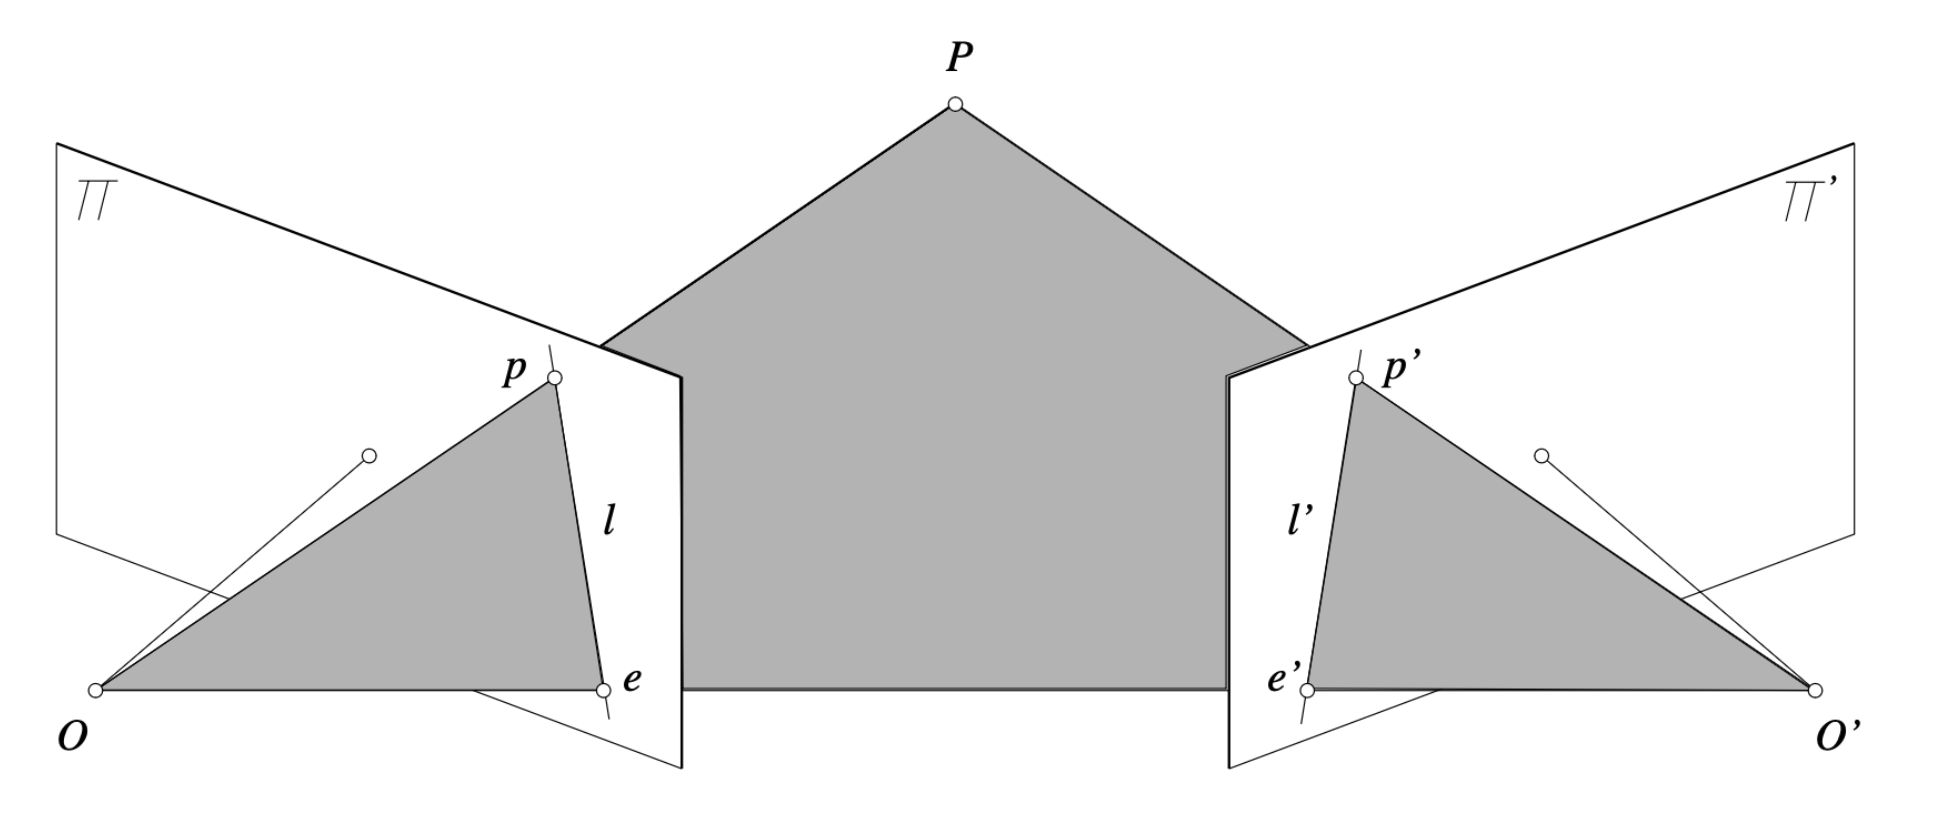
\includegraphics[width=.8\textwidth]{two-view/epipolar-geometry.png}
    \caption{Epipolar geometry.}
    \label{fig:epipolar-geometry}
\end{figure}
The scene is observed from two view points, caracterized by the two optical centers $O$ and $O'$, and their respective projected images (planes $\pi$ and $\pi'$). The line $OO'$ is called the \emph{baseline}, and cuts the planes respectively on $e$ and $e'$ called the \emph{epipoles}. 

The plane formed by $OPO'$ is called the \emph{epipolar plane}. Its intersection with $\pi$ is called the \emph{epipolar line} associated to $p'$, denote $l$. Respectively, its intersection with $\pi'$ is called the epipolar line associated to $p$ and is denoted $l'$.

\begin{remark}
    The epipolar line $l$ is associated with $p'$ and not $p$. This is due to the line $l$ being known whenever $p'$ is.
\end{remark}

\begin{theorem}[Epipolar constraint]
    \label{thm:epipolar-constraint}
    If a point $P$ is observed in two views in $p$ and $p'$, the observation $p$ \textbf{must belong} to the epipolar line associated to $p'$, namely $l$. Respectively, $p'$ must belong to the epipolar line $l'$ associated to $p$.
\end{theorem}

The epipolar constraint (Theorem \ref{thm:epipolar-constraint}) and the geometrical relationship between the two viewpoints' projections can be written as an equation, defining the \emph{Essential Matrix}, introduced by Longuet-Higgins and defined as follows (in the case of known intrinsic parameters):
\begin{equation}
    \label{eq:essential-matrix}
    p\cdot[t\times(\Rc p')]
\end{equation}
where $p=\begin{bmatrix}u\\v\\1\end{bmatrix}$ and $p'=\begin{bmatrix}u'\\v'\\1\end{bmatrix}$ denote the homogeneous coordinates of the observed points in the two view, $t$ is the coordinate vector of the translation $\overrightarrow{OO'}$ and $\Rc$ is the rotation matrix such that a free vector with coordinates $w'$ in the second coordinate system has coordinates $\Rc w'$ in the first coordinate system.

\autoref{eq:essential-matrix} can be rewritten as:
\begin{equation}
    p^\tp\Ec p' = 0
\end{equation}
where $\Ec=[t_\times]\Rc$.\footnote{For any vector $a$, $[a_\times]$ denotes the skew-symmetric matrix such that $[a_\times]b=a\times b$ is the cross-product of the vectors $a$ and $b$.} The matrix $\Ec$ is called the \emph{Essential Matrix}.

\begin{remark}
    Note that in practice, the expression of the essential matrix as $\Ec=[t_\times]\Rc$ does not matter, as we can directly estimate the matrix without computing the rotation and translation matrices. However, in the case of unknown intrinsic camera parameters, the full decomposition, and thus definition, would be different: one would have to compensate for the change of coordinate basis due to different camera parameters for the epipolar constraint to be verified. In this case, the fundamental matrix $F$ is defined such that:
    \begin{equation*}
        (Kp)^\tp F(K'p')=0
    \end{equation*}
    with $K$ and $K'$ the intrinsic parameters of the two cameras.
\end{remark}

\subsection{Essential matrix estimation}
We now assume that we are given a set of corresponding points from views $\pi$ and $\pi'$, with equal intrinsinc parameters, and denoted respectively as $p$ and $p'$. We know that such points must satisfy Theorem \ref{thm:epipolar-constraint}. Therefore, we can use this information to estimate the essential matrix $\Ec$, and use it to make correspondences between new points.

\begin{remark}
    In practice, Longuet-Higgins showed that at least 8 correspondences were needed to have a reasonable estimate of $\Ec$. In these notes, the algorithm is given for one single pair of points $(p,p')$, but it can be easily extended to multiple pairs $(p_i,p_i')_i$.
\end{remark}

Using \autoref{eq:essential-matrix}, we can write the epipolar constraint as:
\begin{equation}
    \begin{bmatrix}u&v&1\end{bmatrix}
    \begin{bmatrix}
        \Ec_{11} & \Ec_{12} & \Ec_{13} \\
        \Ec_{21} & \Ec_{22} & \Ec_{23} \\
        \Ec_{31} & \Ec_{32} & \Ec_{33}
    \end{bmatrix}
    \begin{bmatrix}u'\\v'\\1\end{bmatrix}=0
\end{equation}
which can be rewritten as:
\begin{equation*}
    \begin{bmatrix}
        uu' & uv' & u & vu' & vv' & v & u' & v' & 1
    \end{bmatrix}
    \begin{bmatrix}
        \Ec_{11} & \Ec_{12} & \Ec_{13} & \Ec_{21} & \Ec_{22} & \Ec_{23} & \Ec_{31} & \Ec_{32} & \Ec_{33}
    \end{bmatrix}^\tp=0
\end{equation*}

Similarly to camera calibration, instead of solving this ill-posed problem, Longuet-Higgins proposed to solve the linear least-squares problem:
\begin{equation}
    \label{eq:least-squares-essential}
    \argmin_{\norm{x}^2=1} \norm{Ax}^2
\end{equation}
where $A$ is the matrix of the $8$ correspondences, and $x$ is the vectorized form of $\Ec$. The solution to this approach is given by the singular value decomposition of $A$. Please refer to \autoref{subsec:least-squares-calibration} for more information.

\subsection{Epipolar lines}
In practice, trying to find $\Ec$ such that every point satisfied the epipolar constraint is equivalent to saying that $p$ should belong to the epipolar line associated to $p'$, and vice-versa. In practice, $p$ can be very close but will never exactly belong to the line, as the estimations introduce error. Thus, one might want to compute the average distance from the points to the epipolar lines associated to their respective corresponding points.

Once an estimate of $\Ec$ is obtained, the epipolar line associated to $p'$ is given by:
\begin{equation*}
    l = \Ec p'
\end{equation*}
The distance of a point $x=\begin{bmatrix}
    u\\v\\1
\end{bmatrix}$ to a line $l=\begin{bmatrix}
    a\\b\\c
\end{bmatrix}$ can be written as:
\begin{equation*}
    d(x,l) = \frac{|au+bv+c|}{\sqrt{a^2+b^2}}
\end{equation*}
This measure can give an idea of the quality of the estimate of $\Ec$. However, it is important to visualize the result, and it is necessary to draw the epipolar lines to have a better understanding of the quality of the estimate. For readability and interpretability, it is reasonable to draw segments instead of lines. They shall be centered in the projection of the associated point $p$ on the epipolar line $l$; we denote this projection $\hat{p}$.

Given a point $p=\begin{bmatrix}u\\v\\1\end{bmatrix}$, the projection of $p$ on the line $l=\begin{bmatrix}a\\b\\c\end{bmatrix}$ of direction $L:=\begin{bmatrix}a\\b\\0\end{bmatrix}$ is given by:
\begin{equation*}
    \hat{p} = p - p\cdot l\frac{L}{\norm{L}^2} = p-\frac{p\cdot l}{a^2+b^2}L = p-\frac{au+bv+c}{a^2+b^2}\begin{bmatrix}a\\b\\0\end{bmatrix}
\end{equation*}

Using these two formulae and basic linear algebra allow to recover the epipolar lines, to draw them, and to compute the distance with the points.

\subsection{Hartley's normalization}
The Longuet-Higgins approache described as \autoref{eq:least-squares-essential} is numerically poorly conditioned, and the estimations are often very inaccurate in practice. Hartley thus proposed an improvement of the algorithm, based on a rescaling of the data to ensure that the resulting matrix would satisfy the required properties of the essential or fundament matrix.

The idea is to center the data around 0, and to scale it such that the average distance to the origin is $\sqrt{2}$ (chosen empirically). This is done by applying the following transformation to the points $p$ and $p'$:
\begin{equation*}
    \begin{cases}
        \tilde{p} = Tp\\
        \tilde{p'} = T'p'
    \end{cases}
\end{equation*}
Such matrices $T$ and $T'$ can be computed by:
\begin{equation*}
    T = \begin{bmatrix}
        \sqrt{\frac{2}{\sigma^2}} & 0 & -\sqrt{\frac{2}{\sigma^2}}\mu_x \\
        0 & \sqrt{\frac{2}{\sigma^2}} & -\sqrt{\frac{2}{\sigma^2}}\mu_y \\
        0 & 0 & 1
    \end{bmatrix}
    \quad\text{and}\quad
    T' = \begin{bmatrix}
        \sqrt{\frac{2}{\sigma'^2}} & 0 & -\sqrt{\frac{2}{\sigma'^2}}\mu_x' \\
        0 & \sqrt{\frac{2}{\sigma'^2}} & -\sqrt{\frac{2}{\sigma'^2}}\mu_y' \\
        0 & 0 & 1
    \end{bmatrix}
\end{equation*}
where $\mu_x$ and $\mu_y$ are the average coordinate of $p$, and $\sigma$ is the average distance to the mean (average norm of the vector) for the point $p$.

We can now estimate the solution $\tilde{\Ec}$ by solving the least-squares problem associated with the constraint:
\begin{equation}
    \label{eq:normalized-essential}
    \tilde{p}^\tp\tilde{\Ec}\tilde{p'}=0
\end{equation}

The data having been normalized, it is necessary to impose a constraint on the estimated matrix $\tilde{\Ec}$ such that it respects the properties of the essential matrix: in particular, it should be of rank $2$. To enforce this rank-2 constraint, Hartley proposes to compute the SVD of $\tilde{\Ec}$, such that:
\begin{equation*}
    \tilde{\Ec} = U\Sigma V^\tp
\end{equation*}
where $\Sigma=\diag(r,s,t)$ with $r\leq s\leq t$ the singular values. Replacing $\Sigma$ by $\Sigma'=\diag(s,t,0)$, guarantees that the rank of the matrix is 2. We therefore define:
\begin{equation*}
    \tilde{\Ec}^* = U\Sigma^* V^\tp
\end{equation*}
which is a close estimate of $\tilde{\Ec}$ of rank 2.

From \autoref{eq:normalized-essential}, we can deduce that:
\begin{equation*}
    (Tp)^\tp\tilde{\Ec}^*(T'p')\simeq0
\end{equation*}
and thus, we can recover the final estimate of the essential matrix by projecting back the normalized data to the original coordinate basis:
\begin{equation*}
    \Ec = T^\tp\tilde{\Ec}^*T'
\end{equation*}

In practice, the estimate using Hartley's normalization improves the results by a significant margin, especially for a small number of points (such as 8).
\section{Structure from Motion}

% \section{Epipolar Geometry and Binocular Stereopsis}
% \section{Markov random fields}
\section{Neural Networks for Visual Recognition}
% \section{Mean-shift algorithm for segmentation}
% \section{Multi-view object models}
% \section{Learning methods}


\end{document}